\subsection{Visual Features in Variational Autoencoders}\label{subsec:results_visual_features_in_variational_autoencoders}
The following sections describe the results of the experiments on visual features in variational autoencoders.

\begin{itemize}
    \item Results non-AlexNet-like-VAE on CelebA: especially layer 1 kernels
    \item Results AlexNet-like-VAE on ImageNet: especially layer 1 kernels
    \item Results AlexNet-like image classification CNN on ImageNet: especially layer 1 kernels
    \item Results AlexNet-like-VAE with frozen decoder from classification network
\end{itemize}

\subsubsection{AlexNet Image Classification}
To make sure that the network structure of the \ac{VAE} is apt to generate Gabor wavelets, image classification was performed on ImageNet (see Figure~\ref{fig:alexnet} and Section~\ref{subsec:visual-features-variational-autoencoders} for the used network, see Section~\ref{ssec:imagenet} for ImageNet).
As the accuracy was not of primary concern, the training was stopped during the tenth epoch (\textbf{If time: train all 100 epochs}), the top-1 training accuracy at this time was at 0.85.

\begin{figure}
    \centering
    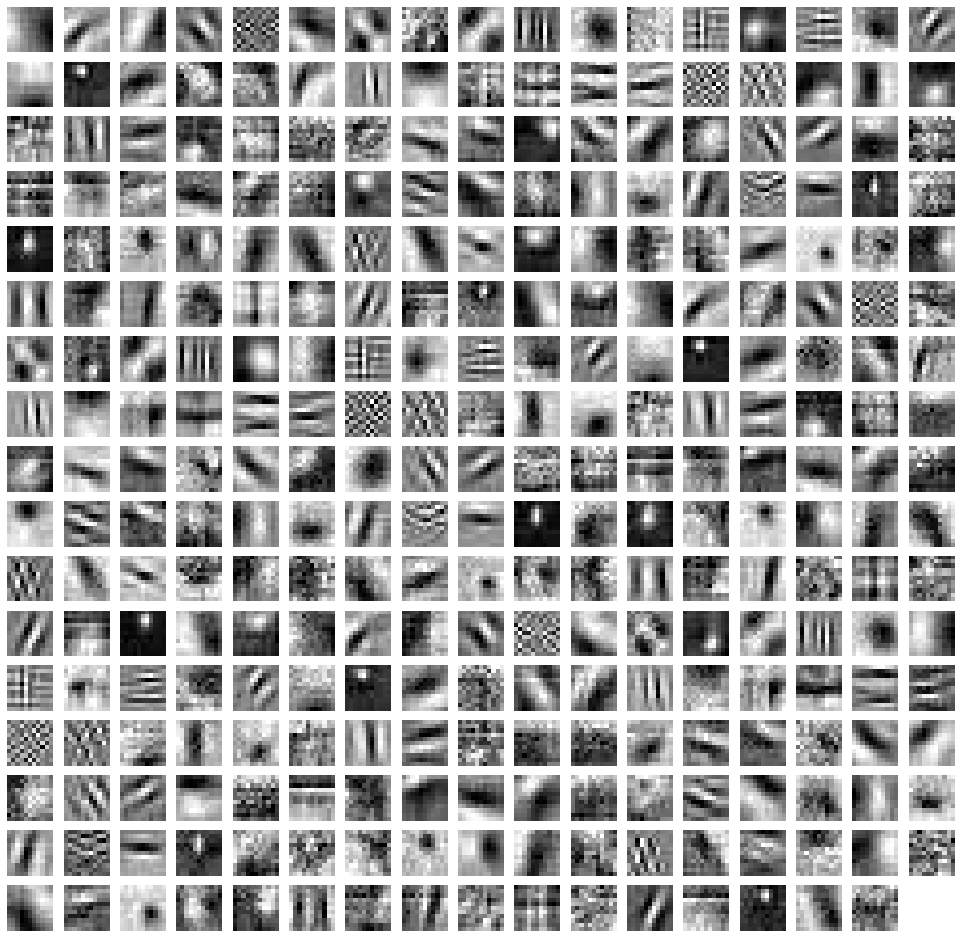
\includegraphics[width=0.9\textwidth]{images/alexnet_classification_l1_kernels.png}
    \caption[Image classification - Layer 1 Kernels]{Convolutional Kernels in the first layer of the image classification network. The filters are shown in their original size (11x11).}
    \label{fig:classification_layer1_kernels}
\end{figure}

Figure~\ref{fig:classification_layer1_kernels} shows all 256 convolutional kernels of the image classification network.
It is easy to see that in many kernels, Gabor wavelet-like filters emerge.

\subsection{V(L)AE Generated Samples vs. True Samples}\label{subsec:vae-generated-samples-vs-true-samples}
\acp{GAN} (see Section~\ref{subsubsec:representation_learning}) are trained by simulatenously training a \textit{generator} to create new samples and a \textit{discriminator} to discriminate between true and generated samples.
\acp{VAE} are another generative model that is not forced in the same way to create indistinguishable samples.
Instead, a reconstruction loss is used to force the reconstruction to be close to the true sample in terms of difference in the pixel values.
At the same time, the \ac{KL}-loss and the reparametrization trick force the model to place similar samples close toanother in a continuous Gaussian embedding space.
Drawing from the Gaussian embedding space therefore should allow to generate new samples similar to true samples.
However, the question remains how indistinguishable these generates samples are from true samples.

To address this question, different statistical analyses were performed revealing that in fact VAE generated samples can be perfectly distinguished from true samples.
\textbf{Talk about the blurriness in VAE generated samples that are another strong reason why this is possible.}

\begin{figure}
    \centering
    \begin{subfigure}{0.4\textwidth}
        \centering
        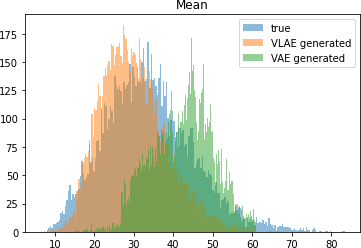
\includegraphics[width=\textwidth]{images/vlae_generated_vs_true/mnist_vs_vlae_mean.png}
        \caption{Mean}
        \label{subfig:vlae_mean_generated_vs_true}
    \end{subfigure}
    \hfill
    \begin{subfigure}{0.4\textwidth}
        \centering
        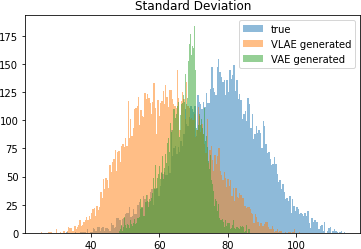
\includegraphics[width=\textwidth]{images/vlae_generated_vs_true/mnist_vs_vlae_sd.png}
        \caption{Standard Deviation}
        \label{subfig:vae_sd_generated_vs_true}
    \end{subfigure}
    \hfill
    \begin{subfigure}{0.4\textwidth}
        \centering
        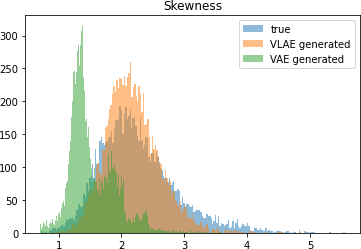
\includegraphics[width=\textwidth]{images/vlae_generated_vs_true/mnist_vs_vlae_skew.png}
        \caption{Skewness}
        \label{subfig:vae_skew_generated_vs_true}
    \end{subfigure}
    \hfill
    \begin{subfigure}{0.4\textwidth}
        \centering
        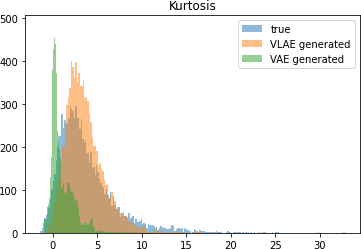
\includegraphics[width=\textwidth]{images/vlae_generated_vs_true/mnist_vs_vlae_kurt.png}
        \caption{Kurtosis}
        \label{subfig:vae_kurt_generated_vs_true}
    \end{subfigure}
    \caption{Comparison of image statistics of \ac{VAE} and \ac{VLAE} compared to \textsc{MNIST} test images. }
    \label{fig:mean_generated_vs_true}
\end{figure}


The MNIST test set of 10,000 images was compared to a 10.000 generated samples from the Vanilla \ac{VAE} and the \ac{VLAE}.
The samples were generated by drawing from a standard two-dimensional Gaussian distribution $\mathcal{N}^2(\bm{0},\bm{I})$.
First, the mean pixel values, i.e.~the mean over all $28\times 28$ pixel values, were compared (see Figure~\ref{subfig:vlae_mean_generated_vs_true}).
The plot overlays the histograms of mean pixel values for the three conditions: \textsc{MNIST}, \ac{VAE}, and \ac{VLAE}.
The other plots in Figure~\ref{fig:mean_generated_vs_true} were created accordingly but for higher moments of the pixel value distributions.

Analyzing Figure~\ref{fig:mean_generated_vs_true} leads to the assumption that, except for Figure~\ref{subfig:vae_sd_generated_vs_true}, the \ac{VLAE} captures the statistics better than the \ac{VAE}.
\begin{table}
    \begin{tabular}{lrrrr}
        \toprule
        Model & $p$-value (mean) & $p$-value (sd) & $p$-value (skewness) & $p$-value (kurtosis)\\
        \midrule
        \ac{VAE} & 0.0 & 0.0 & 0.0 & 0.0 \\
        \ac{VLAE} & $1.8\cdot 10^{-147}$ & 0.0 & $7.9\cdot 10^{-11}$ & 0.309\\
        \bottomrule
    \end{tabular}
    \caption{$p$-values of a Wilcoxon signed-rank test. Each cell tests the hypothesis that the respective moments for the respective model are equal to the values for the \textsc{MNIST} test images. For each cell, the sample size was $2\cdot 10,000$.}
    \label{tab:vae-vlae-mnist}
\end{table}
Table~\ref{tab:vae-vlae-mnist} shows the results of a Wilcoxon signed-rank test for the samples of moments of the pixel distributions.
The results lead to two conclusions: 1) The \ac{VLAE} in fact captures the statistics of the pixel distribution better compared to the \ac{VAE}.
2) Both models do not capture the true pixel distribution.

Similar to the \ac{GAN} approach, a discriminator network was trained to distinguish generated samples from true \textsc{MNIST} test images\footnote{The configuration of the discriminator network can be found in Appendix \ref{sec:listing_discriminator_network}.}.
The discriminator network shows an accuracy of 1.0 for distinguishing both, \ac{VAE} generated from \textsc{MNIST} test images as well as  \ac{VLAE} from \textsc{MNIST} test images.

\subsection{Independence of VLAE Embeddings}\label{subsec:independence-of-vlae-embeddings}

\begin{figure}[t]
    \centering
    \begin{subfigure}{0.3\textwidth}
        \centering
        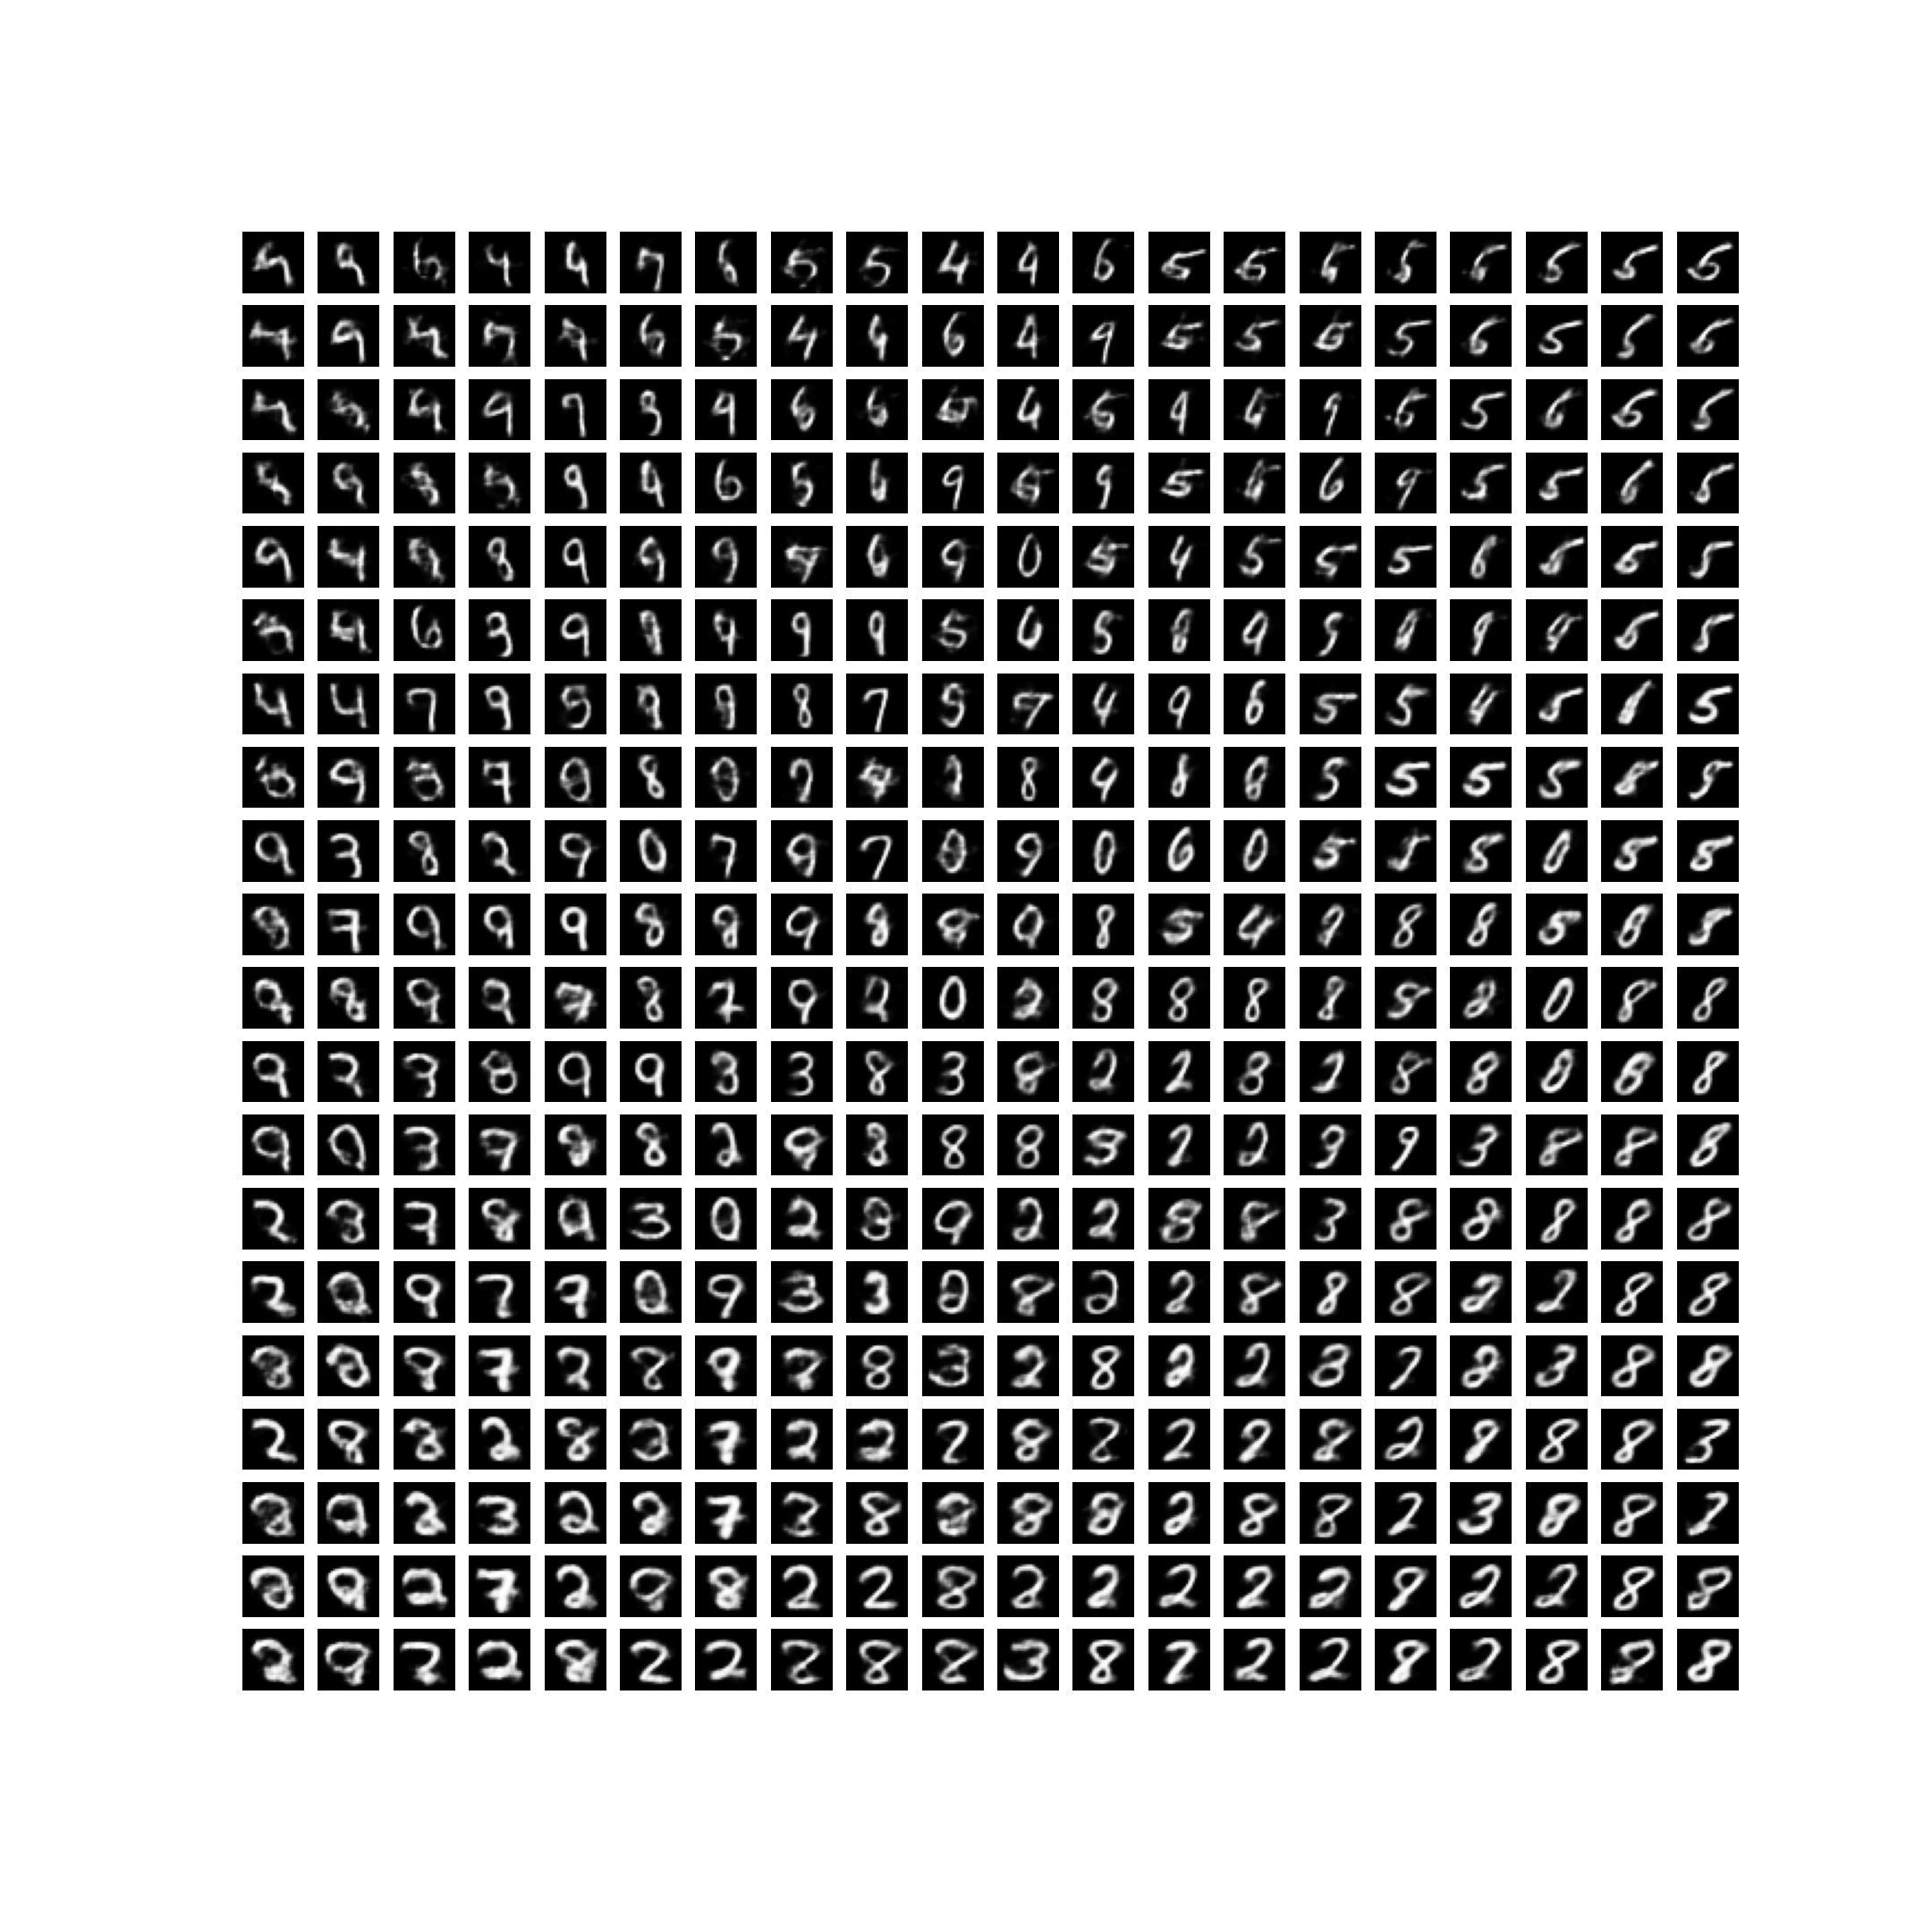
\includegraphics[width=\textwidth]{images/vlae_plots1.png}
        \caption{Exploring $z_1$}
        \label{subfig:vlae_plots1}
    \end{subfigure}
    \hfill
    \begin{subfigure}{0.3\textwidth}
        \centering
        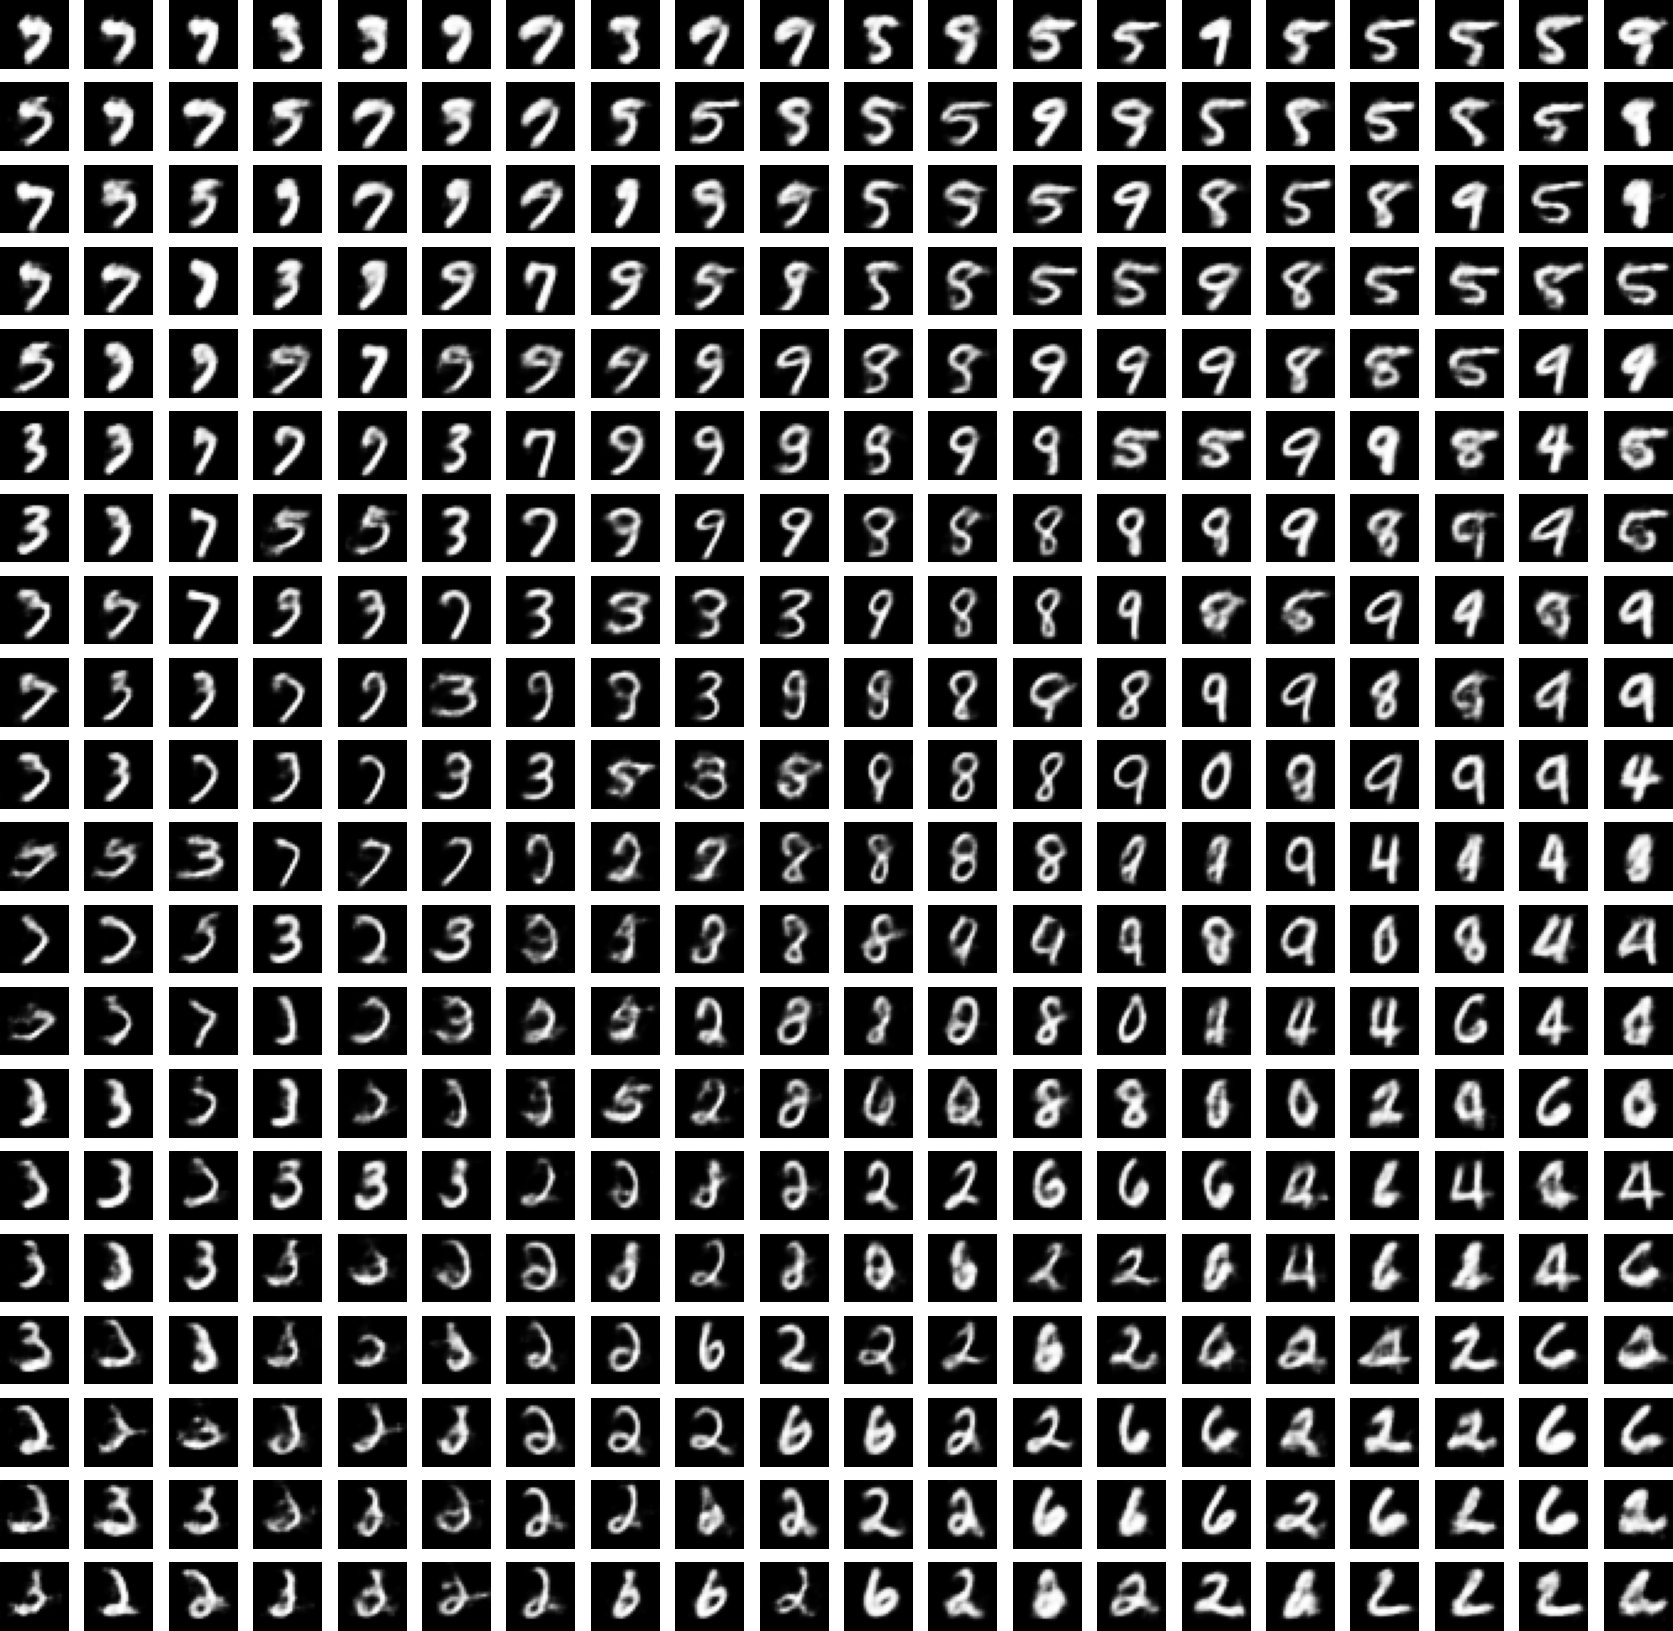
\includegraphics[width=\textwidth]{images/vlae_plots2.png}
        \caption{Exploring $z_{2}$}
        \label{subfig:vlae_plots2}
    \end{subfigure}
    \hfill
    \begin{subfigure}{0.3\textwidth}
        \centering
        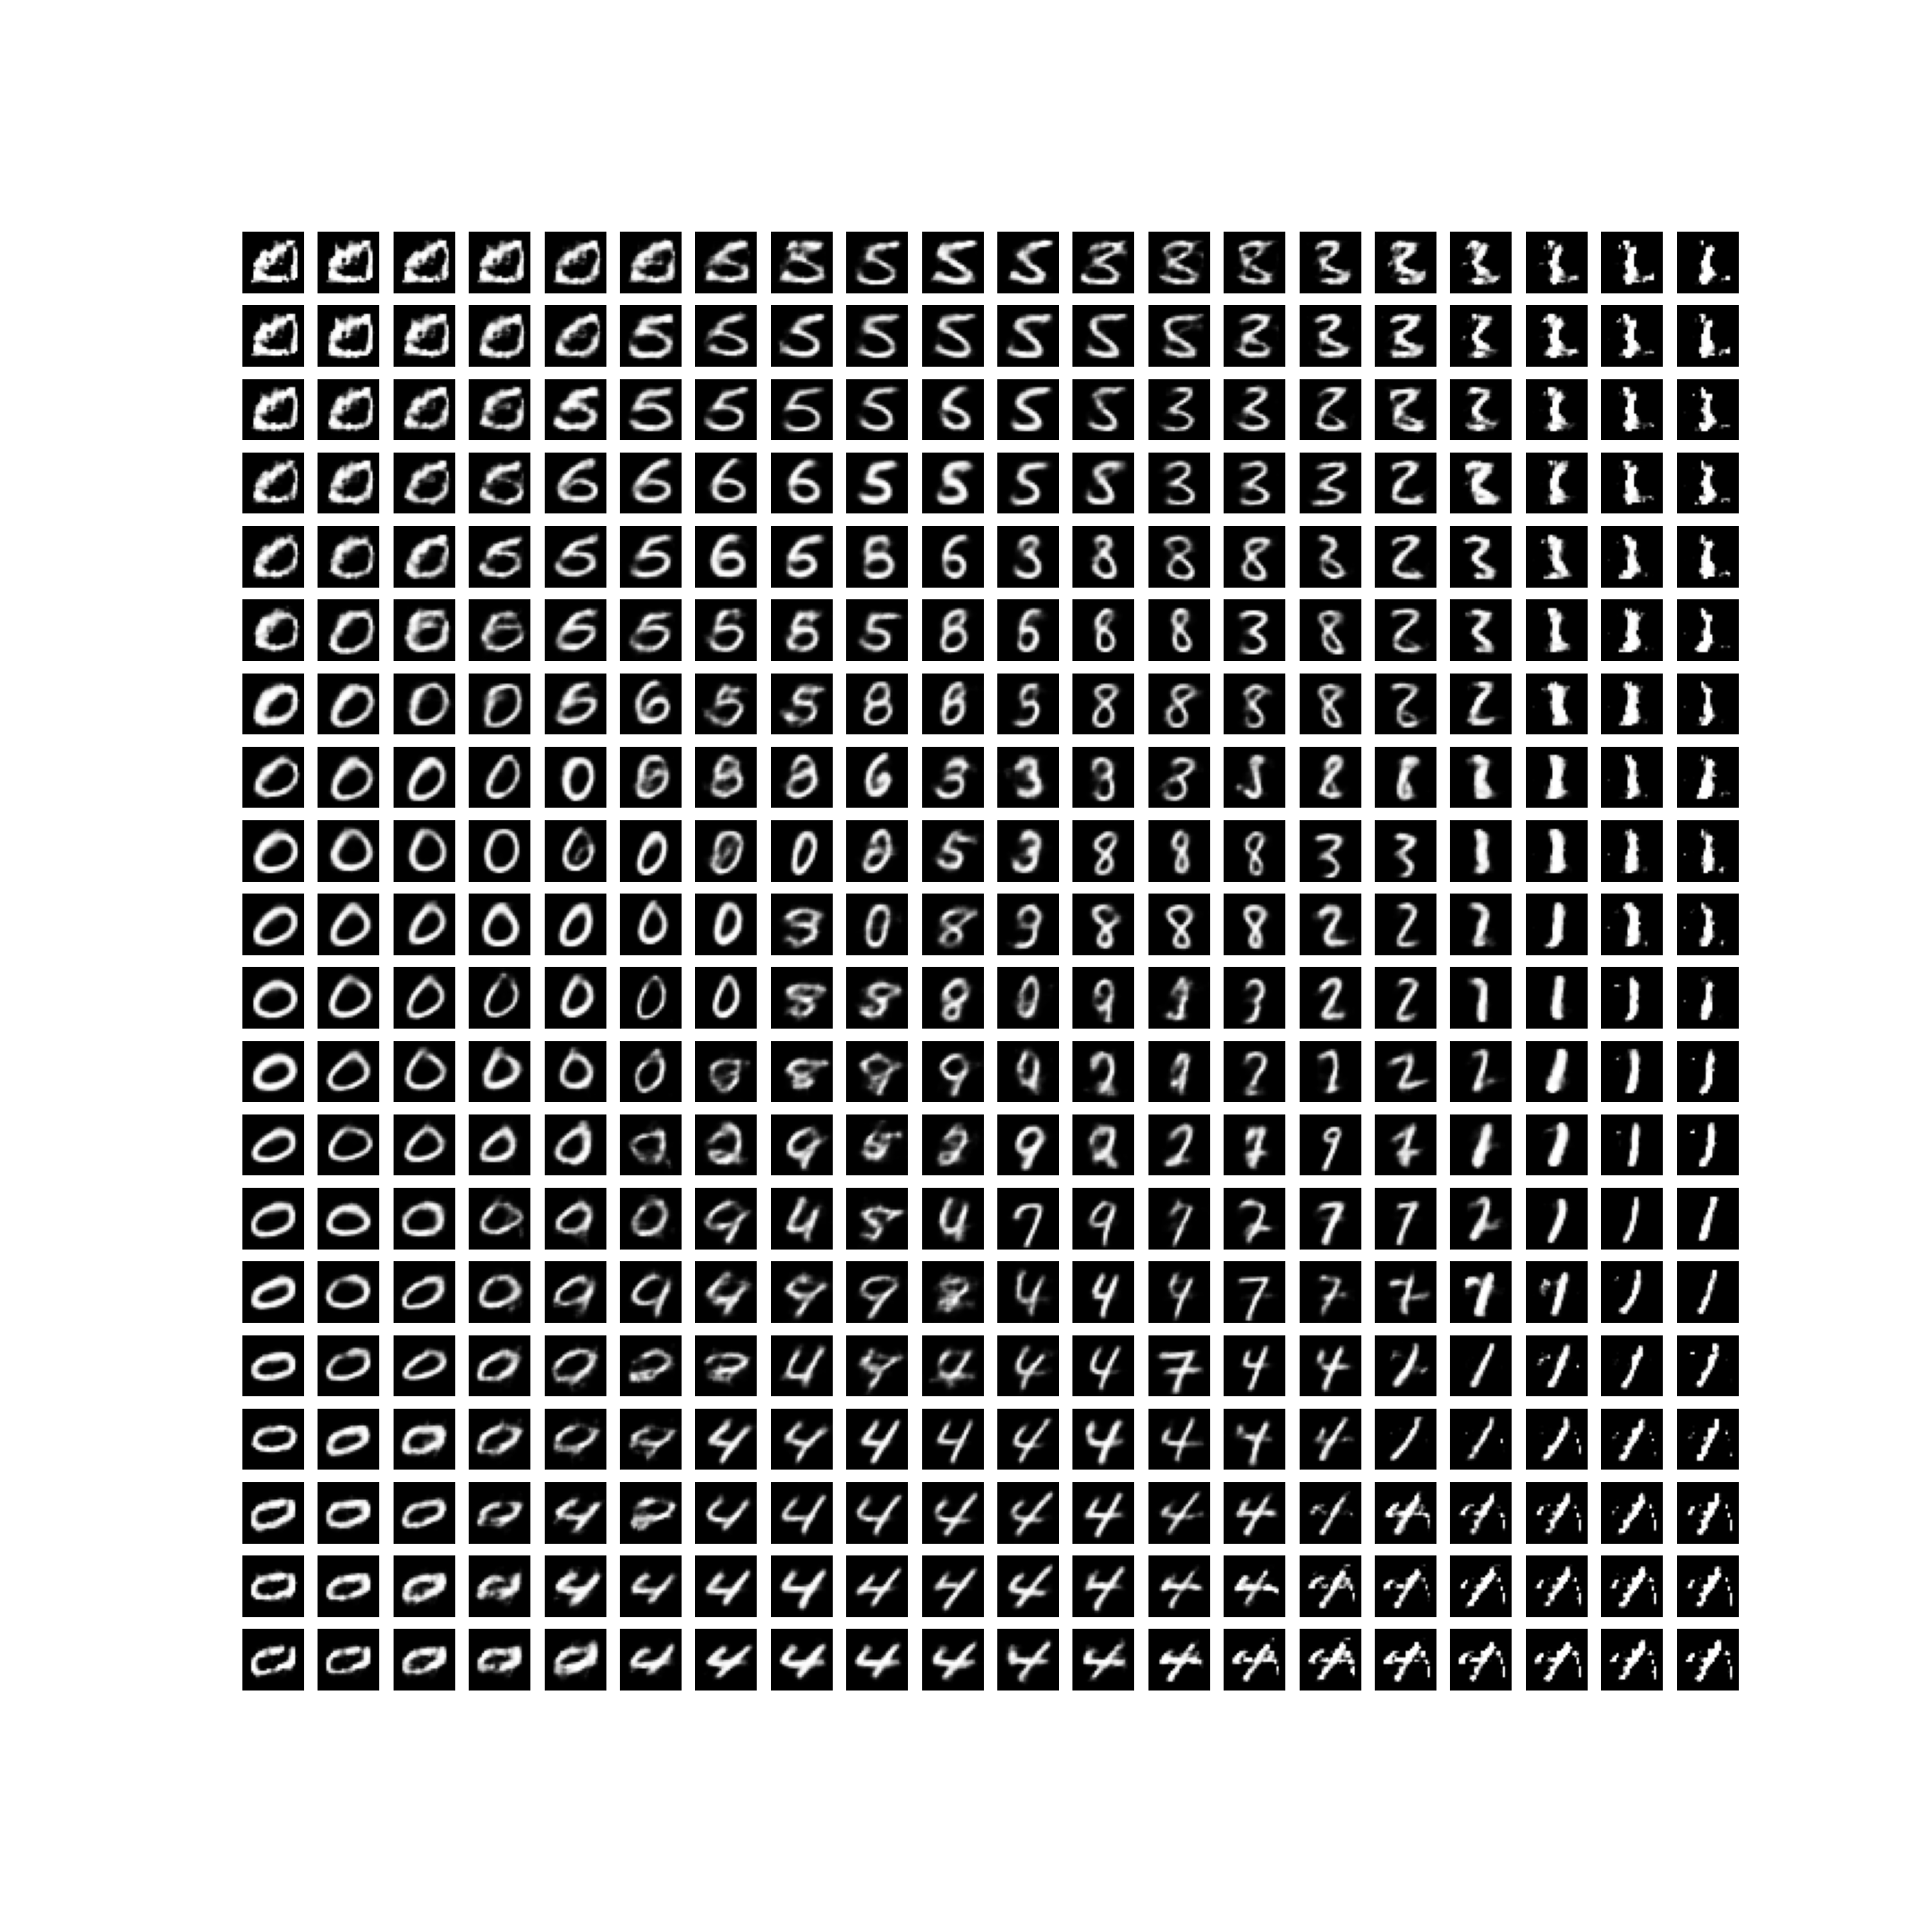
\includegraphics[width=\textwidth]{images/vlae_plots3.png}
        \caption{Exploring $z_3$}
        \label{subfig:vlae_plots3}
    \end{subfigure}
    \caption{Reconstructions of the VLAE model when systematically exploring one latent space and randomly choosing the other two latent spaces. The space explored systematically is sampled from -3 SD to 3 SD in both dimensions, the other values are chosen by drawing from an uniform distribution over $[-1; 1]$. Created analogously to \citet[Figure 5]{zhao2017learning}.}
    \label{fig:vlae_plots}
\end{figure}
The VLAE learns embeddings on different levels.
For MNIST, \citet{zhao2017learning} used three two-dimensional layers to learn image semantics of different granularity.
They claim that their model is able to learn disentangled hierarchical features.
Figure~\ref{fig:vlae_plots} shows reconstructions of this model when systematically exploring one dimensions and randomly choosing the others.
Apparently, the model is able to learn disentangled representations to some extent.

For example, $z_1$ seems to mainly encode the digit orientation, $z_2$ seems to primarily encode digit width, whereas $z_3$ seems to encode digit identity.
However, it is not obvious how disentangled the representations actually are.
\begin{breakablealgorithm}
    \caption{Generating Layer Representative Samples by Averaging Out Other Embedding Layers}\label{alg:layer_representative_samples}
    \begin{algorithmic}[1]
        \Function{LayerRepresentativeSamples}{numSamples,numApproximations}
        \State $j \gets 0$
        \State $\mathcal{L}\gets \varnothing$
        \While{$i < \text{numSamples}$}
        \State $\bm{v} \gets \bm{v} \sim \mathcal{N}(\bm{0}, \bm{I})$\label{line:fixing_v}
        \ForAll{$j \in \{1,2,3\}$}
        \State $\bm{s}_j \gets$ \Call{LayerRepresentativeSample}{$\bm{v}$, numApproximations, $j$}
        \EndFor
        \State $\mathcal{L} \gets \mathcal{L} \cup \{\{\bm{s}_1, \bm{s}_2, \bm{s}_3\}\}$

        \EndWhile
        \State \Return $\mathcal{L}$
        \EndFunction

        \Function{LayerRepresentativeSample}{fixedDimensionValue, numApproximations, dimensionIndex}
        \State $\mathcal{D} \gets \{1,2,3\}$
        \State $\alpha \gets \text{fixedDimensionValue}$
        \State $\beta \gets (D \setminus \text{dimensionIndex})_1$
        \State $\gamma \gets (D \setminus \text{dimensionIndex})_2$
        \State $\bm{z}_{\alpha} \gets \bm{a} \sim \mathcal{N}(\bm{0}, \bm{I})$
        \State $\mathcal{L}\gets \varnothing$
        \State $i \gets 0$
        \While{$i < \text{numApproximations}$}
        \State $\bm{z}_{\beta}^i \gets \bm{b}_i \sim \mathcal{N}(\bm{0}, \bm{I})$
        \State $\bm{z}_{\gamma}^i \gets \bm{c}_i \sim \mathcal{N}(\bm{0}, \bm{I})$
        \State $\mathcal{L} \gets \mathcal{L} \cup \{$ \Call{VLAE-Decoder}{$\bm{z}_{\alpha}, \bm{z}_{\beta}^j, \bm{z}_{\gamma}^j$} $\}$
        \State $i \gets i + 1$
        \EndWhile
        \State \Return $\frac{1}{|\mathcal{L}|}\sum_j \mathcal{L}_j$
        \EndFunction
    \end{algorithmic}
\end{breakablealgorithm}

Consider Algorithm~\ref{alg:layer_representative_samples}.
The function call \textsc{VLAE-Decoder} calls the decoder of the VLAE, i.e. $p_\theta(\bm{x} | \bm{z}_1, \bm{z}_2, \bm{z}_3)$.
Calling the function \textsc{LayerRepresentativeSamples} returns an ordered set $\mathcal{L}$ of \say{layer representative samples}.
Each sample $i$ contains three items, say $\bm{x}_1^i, \bm{x}_2^i, \bm{x}_3^i$ that were created by fixing a value $\bm{v}$ in Line~\ref{line:fixing_v} of Algorithm \ref{alg:layer_representative_samples}.
What is meant by the term \say{layer representative samples} is that for example $\bm{x}_1^i$ is approximately drawn from the marginal distribution
\begin{align}
    \bm{x}_1^i \sim p_\theta(\bm{v} | \bm{z}_1) = \int_{\bm{z}_2} \int_{\bm{z}_3} p_\theta(\bm{v} | \bm{z}_1, \bm{z}_2, \bm{z}_3) d\bm{z}_2 d\bm{z}_3
\end{align}
Now, if the embedding layers learn disentangled hierarchical representations, $p_\theta(\bm{x} | \bm{z}_1)$, $p_\theta(\bm{x} | \bm{z}_2)$, and $p_\theta(\bm{x} | \bm{z}_3)$ should be pairwise statistically independent.
Specifically,
\begin{align}
    p_\theta(\bm{x} | \bm{z}_i) \not \propto p_\theta(\bm{x} | \bm{z}_j) \quad \forall (i,j):i\neq j \label{eq:notprop}
\end{align}

\begin{figure}
    \centering
    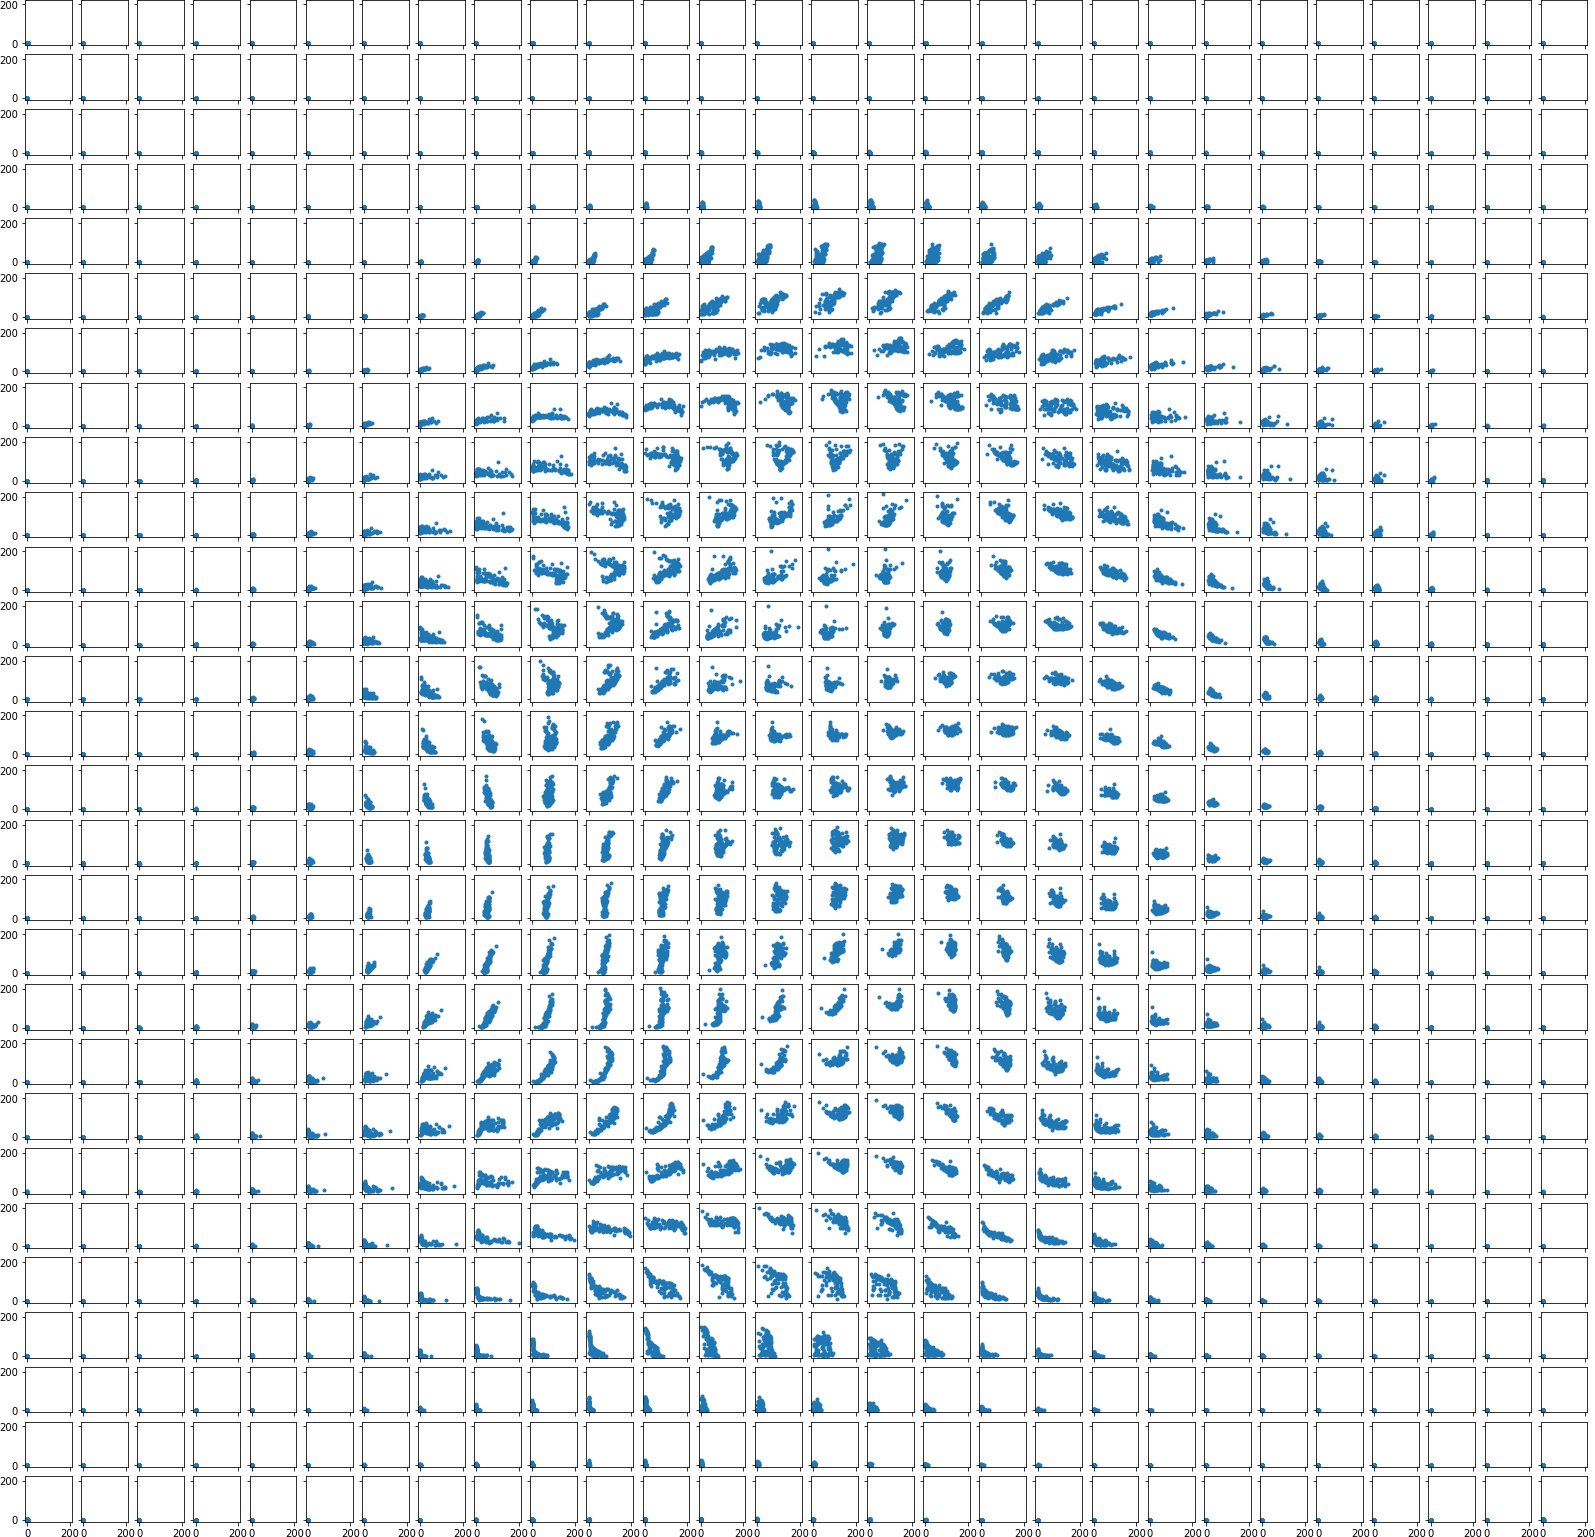
\includegraphics[width=\textwidth]{images/notprop.png}
    \caption{Proportionality of pixel intensities when fixing $\bm{z}_1 = \bm{z}_2=\varphi$. Each box represents one of $28\times 28$ MNIST pixels. The $x$-axis of each box encodes the mean pixel intensity of the $\bm{z}_1$-representative sample. The $y$-axis encodes the mean pixel intensity of the of the $\bm{z}_2$-representative sample. Dots within boxes belong to the same $\varphi$ for both, $\bm{z}_1$ and $\bm{z}_2$. }
    \label{fig:notprop}
\end{figure}

However, this is not true.
Choosing a value $\bm{z}_1 = \varphi$ such that $p_\theta(\bm{x} | \bm{z}_1 = \varphi)$ also leads to a high value of $p_\theta(\bm{x} | \bm{z}_2 = \varphi)$, leading to a violation of Equation \ref{eq:notprop}.

Consider Figure~\ref{fig:notprop}.
It shows results of samples $(\bm{x}_1^1,\bm{x}_2^1),\dots,(\bm{x}_1^{100},\bm{x}_{100}00)$ that were generated by Algorithm~\ref{alg:layer_representative_samples}\footnote{The results for the other combinations, $(\bm{z}_1,\bm{z}_3)$ and $(\bm{z}_2,\bm{z}_3)$ can be found in Appendix \ref{sec:additional-plots-for-section_independence}}.
Thus, the parameter \say{numSamples} is chosen as 100 and the parameter \say{numApproximations} is chosen as 300.
Each $\bm{x}_i^j$ is one generated MNIST image of size $28\times 28$ pixels.
Each box in Figure~\ref{fig:notprop} corresponds to one of these pixels, the box index corresponds to the pixel in the MNIST image.
The $x$-values of dots in the same box then correspond to $\bm{x}_1^1\big|_{(3,1)}, \dots, \bm{x}_1^{100}\big|_{(3,1)}$, i.e. the pixel intensities of one specific pixel (here: third row, first column (3,1)) over all 100 samples for $\bm{x}_1$, i.e. the sample generated by fixing $\bm{z}_1$.
Analogously, the $y$-values of dots in the same box correspond to $\bm{x}_2^1\big|_{(3,1)}, \dots, \bm{x}_2^{100}\big|_{(3,1)}$.
Each dot corresponds to one fixed $\varphi$-value.

Now, if changing the value of $\bm{z}_1$ was independent of changing the value of $\bm{z}_2$, the boxes should show now trend.
This is true for outer boxes.
They correspond to pixel values that always close to zero, therefore the value are in the bottom left corner and no correlation can be observed.
For center pixels, however, the plot shows something different.
They show an interesting correlation pattern of negative and positive correlations.

Negative correlations for a pixel with index $(i,j)$ indicate that $p_\theta(\bm{x}\big|_{(i,j)} | \bm{z}_1 = \varphi) \propto \frac{1}{p_\theta(\bm{x}\big|_{(i,j)} | \bm{z}_1 = \varphi)}$, i.e. choosing a value $\varphi$ that leads to a high $(i,j)$-pixel intensity for the $\bm{z}_1$-representative sample leads to a low intensity of the same pixel of the corresponding $\bm{z}_1$-representative sample.
This, however, is a violation of equation~\ref{eq:notprop}.
Importantly, the correlation only persists for certain pixels.

\textbf{Investigate, if possible, this in terms of Perceptual Path Length and Linear Separability (see \citet{karras2019style}).}

\subsection{Morpho-MNIST on VLAE}\label{subsec:morpho-mnist-on-vlae}

As discussed in Section~\ref{subsubsec:representation_learning}, the \acl{VLAE} aims at learning \say{hierarchical disentangled representation}~\citep{zhao2017learning}.
The lower embedding layers of such a model trained on MNIST (see Section~\ref{subsubsec:mnist}) encode features such as stroke width, digit width, and digit tilt whereas the highest layer mainly learns digit identity~\citep{zhao2017learning}.

\begin{figure}
    \centering
    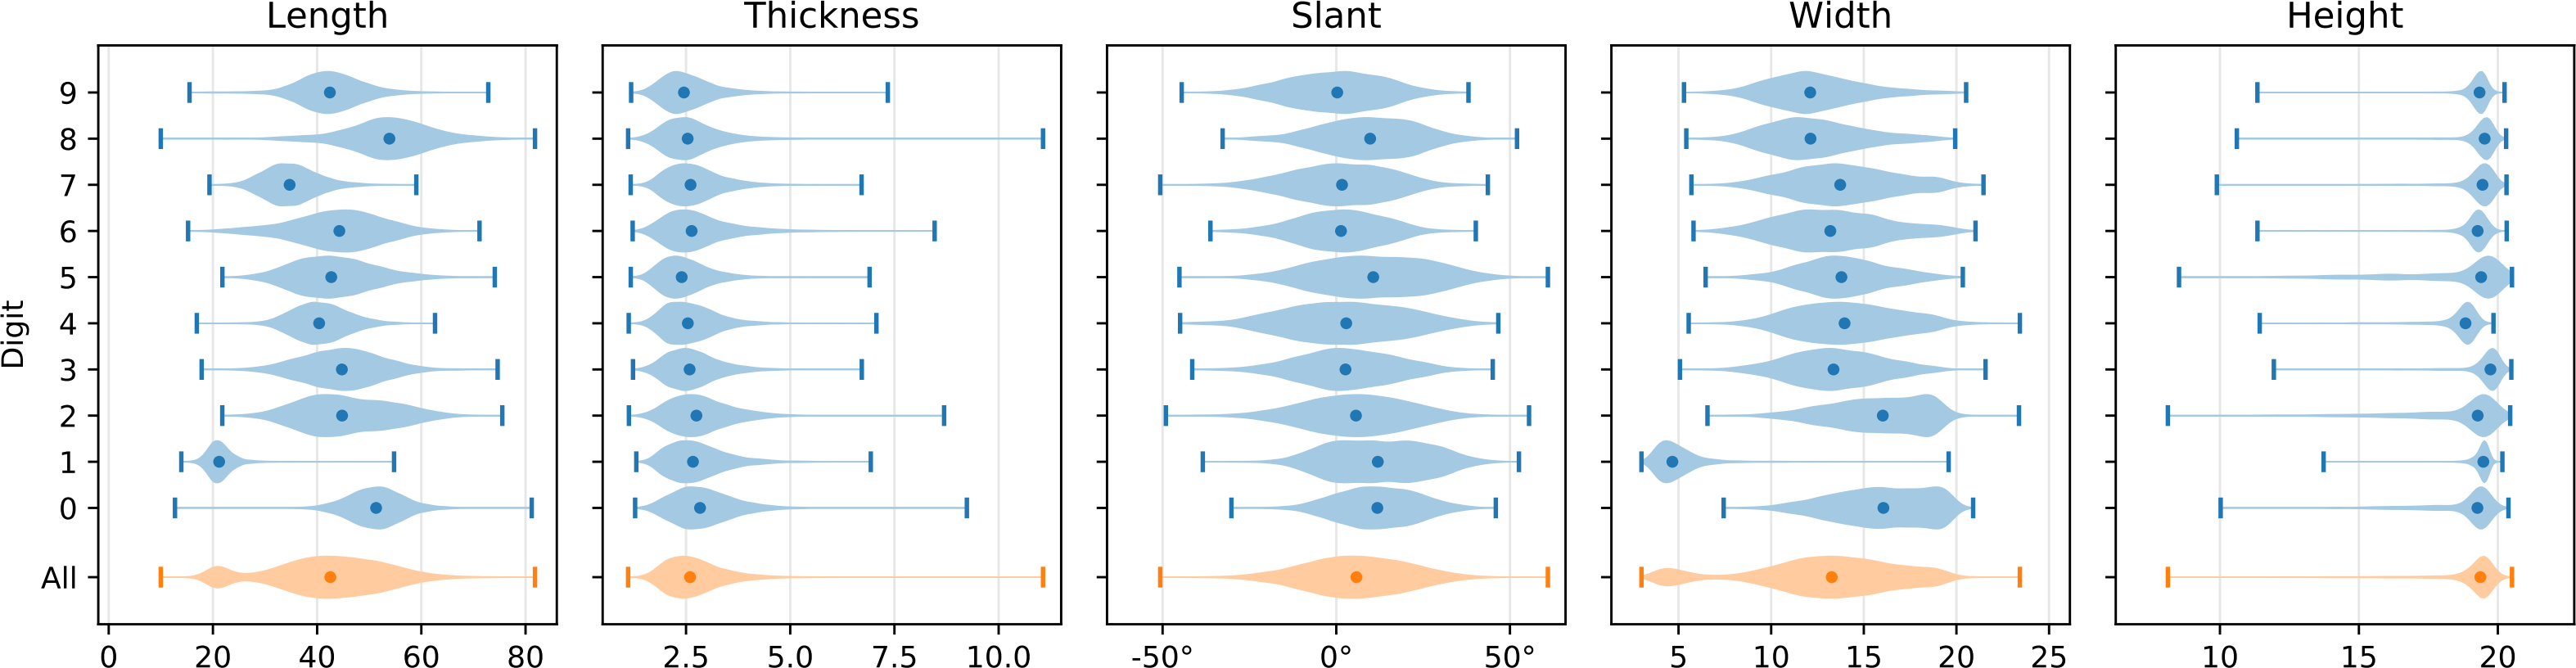
\includegraphics[width=\textwidth]{images/morpho_mnist_distribution.png}
    \caption{Distribution of the \textsc{Morpho-MNIST} attributes for the different digits. Taken from \citep{castro2019morpho}.}
    \label{fig:morpho_mnist_distribution}
\end{figure}

Incorporating the additional labels provided by Morpho-\textsc{MNIST} (see Section~\ref{subsubsec:morphomnist}) helps to analyze to what extent the lower layers learn which morphological features of \textsc{MNIST}.
The morphological attributes, however, are not equally distributed for all digits.
The mean stroke length and the digith width, for example, have a very low mean value for the digit \say{1} (see Figure~\ref{fig:morpho_mnist_distribution}).
Therefore, it should be possible to almost uniquely identify the identity of the digit \say{1} by just considering the stroke length or the digit width.
Other attributes such as stroke thickness, digit slant, and digit height are more evenly distributed (see Figure~\ref{fig:morpho_mnist_distribution}).

\begin{figure}
    \centering
    \begin{subfigure}{.33\textwidth}
        \centering
        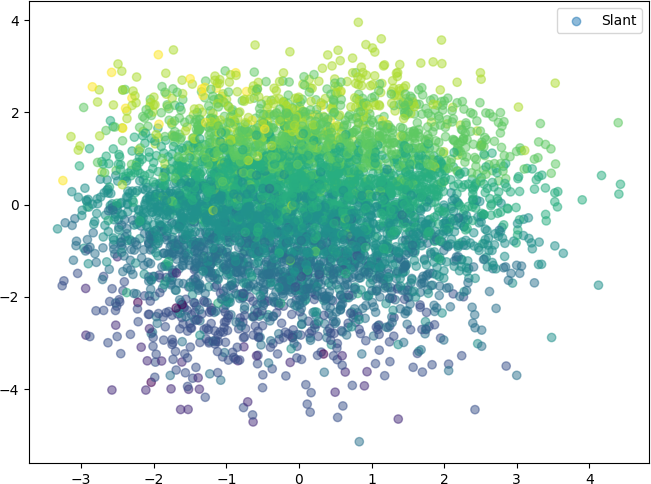
\includegraphics[width=\textwidth]{images/vlae_embeddings/embeddings_mu_1_0.png}
        \caption{}
        \label{fig:vlae_embeddings_mu1_slant}
    \end{subfigure}%
    \begin{subfigure}{.33\textwidth}
        \centering
        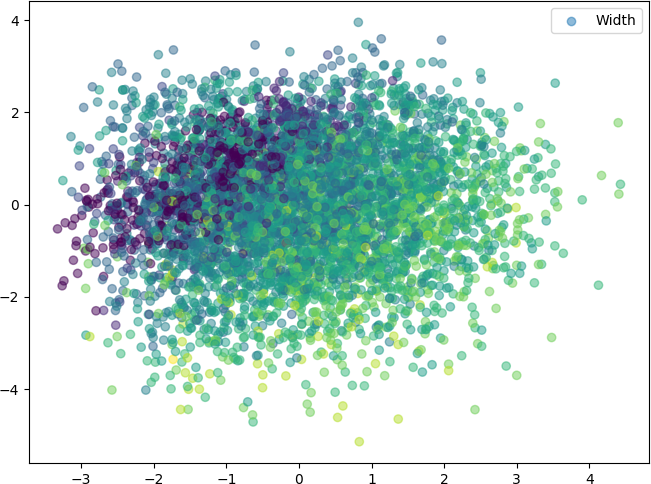
\includegraphics[width=\textwidth]{images/vlae_embeddings/embeddings_mu_1_4.png}
        \caption{}
        \label{fig:vlae_embeddings_mu1_width}
    \end{subfigure}
    \begin{subfigure}{.33\textwidth}
        \centering
        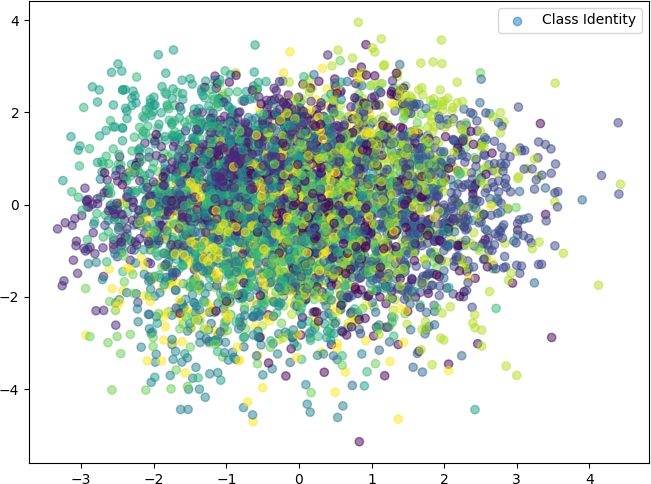
\includegraphics[width=\textwidth]{images/vlae_embeddings/embeddings_mu_1_6.png}
        \caption{}
        \label{fig:vlae_embeddings_mu1_identity}
    \end{subfigure}
    \caption{5000 random training points plotted in the first embedding layer $\bm{z}_1$ for the VLAE model. The position of the dots does not change in the diffent subplot. Different color dots by different means (shown in the respective legend). The morphological attributes are evenly assigned to ten bins. Dark colors indicate a low value of the respective whereas bright colors indicate a high value.}
    \label{fig:vlae_embeddings_mu1}
\end{figure}

Consider Figure~\ref{fig:vlae_embeddings_mu1_slant} showing the embedding layer $\bm{z}_1$ colored by digit slant\footnote{A complete plot of all morphological attributes for all layers can be found in Appendix~\ref{sec:additional-plots-for-section_morpho_mnist}.}.
Figure~\ref{fig:morpho_mnist_distribution} shows that the mean of the attribute \textit{Slant} is quite evenly distributed.
The color gradient in Figure~\ref{fig:vlae_embeddings_mu1_slant} therefore indicates that the VLAE actually learns the morphological attribute instead of just showing the class identity, encoded by means of another morphological attribute that correlates with class identity.

For Figure~\ref{fig:vlae_embeddings_mu1_width}, the situation is different.
The noticeable dark-purple cluster in the top left correlates with dark-purple points in Figure~\ref{fig:vlae_embeddings_mu1_identity} that encode image with label \say{1}.
For digit width, however, \say{1} is an outlier (see Figure~\ref{fig:morpho_mnist_distribution}) and a small digit width therefore is a strong indicator for a digit identity of \say{1}.
Not considering the dark-purple points, $\bm{z}_1$ still shows a less prominent color gradient from the bottom right to the top left.
In contrast, digit identity does not seem to be encoded strongly by $\bm{z}_1$ (see Figure~\ref{fig:vlae_embeddings_mu1_identity}).

\textbf{continue}

\subsection{Sparse Activations}
\textbf{DRAFT!}
Present results on feature map activities: most inactive, only a few active.
\citet{yoshida2020natural} show that natural images are sparsely encoded in mice V1, however in contrast to our results, the overlap for different images is quite small.
Discuss the implications on the model suitability.

\subsection{Feature Map Stripes}\label{subsec:feature-map-stripes}

\begin{figure}
    \centering
    \begin{subfigure}{0.3\textwidth}
        \centering
        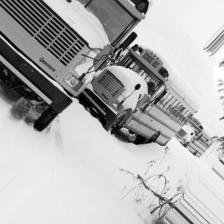
\includegraphics[width=\textwidth]{images/stripes/original.jpg}
        \caption{The original image.}
        \label{subfig:stripes_original}
    \end{subfigure}
    \hfill
    \begin{subfigure}{0.3\textwidth}
        \centering
        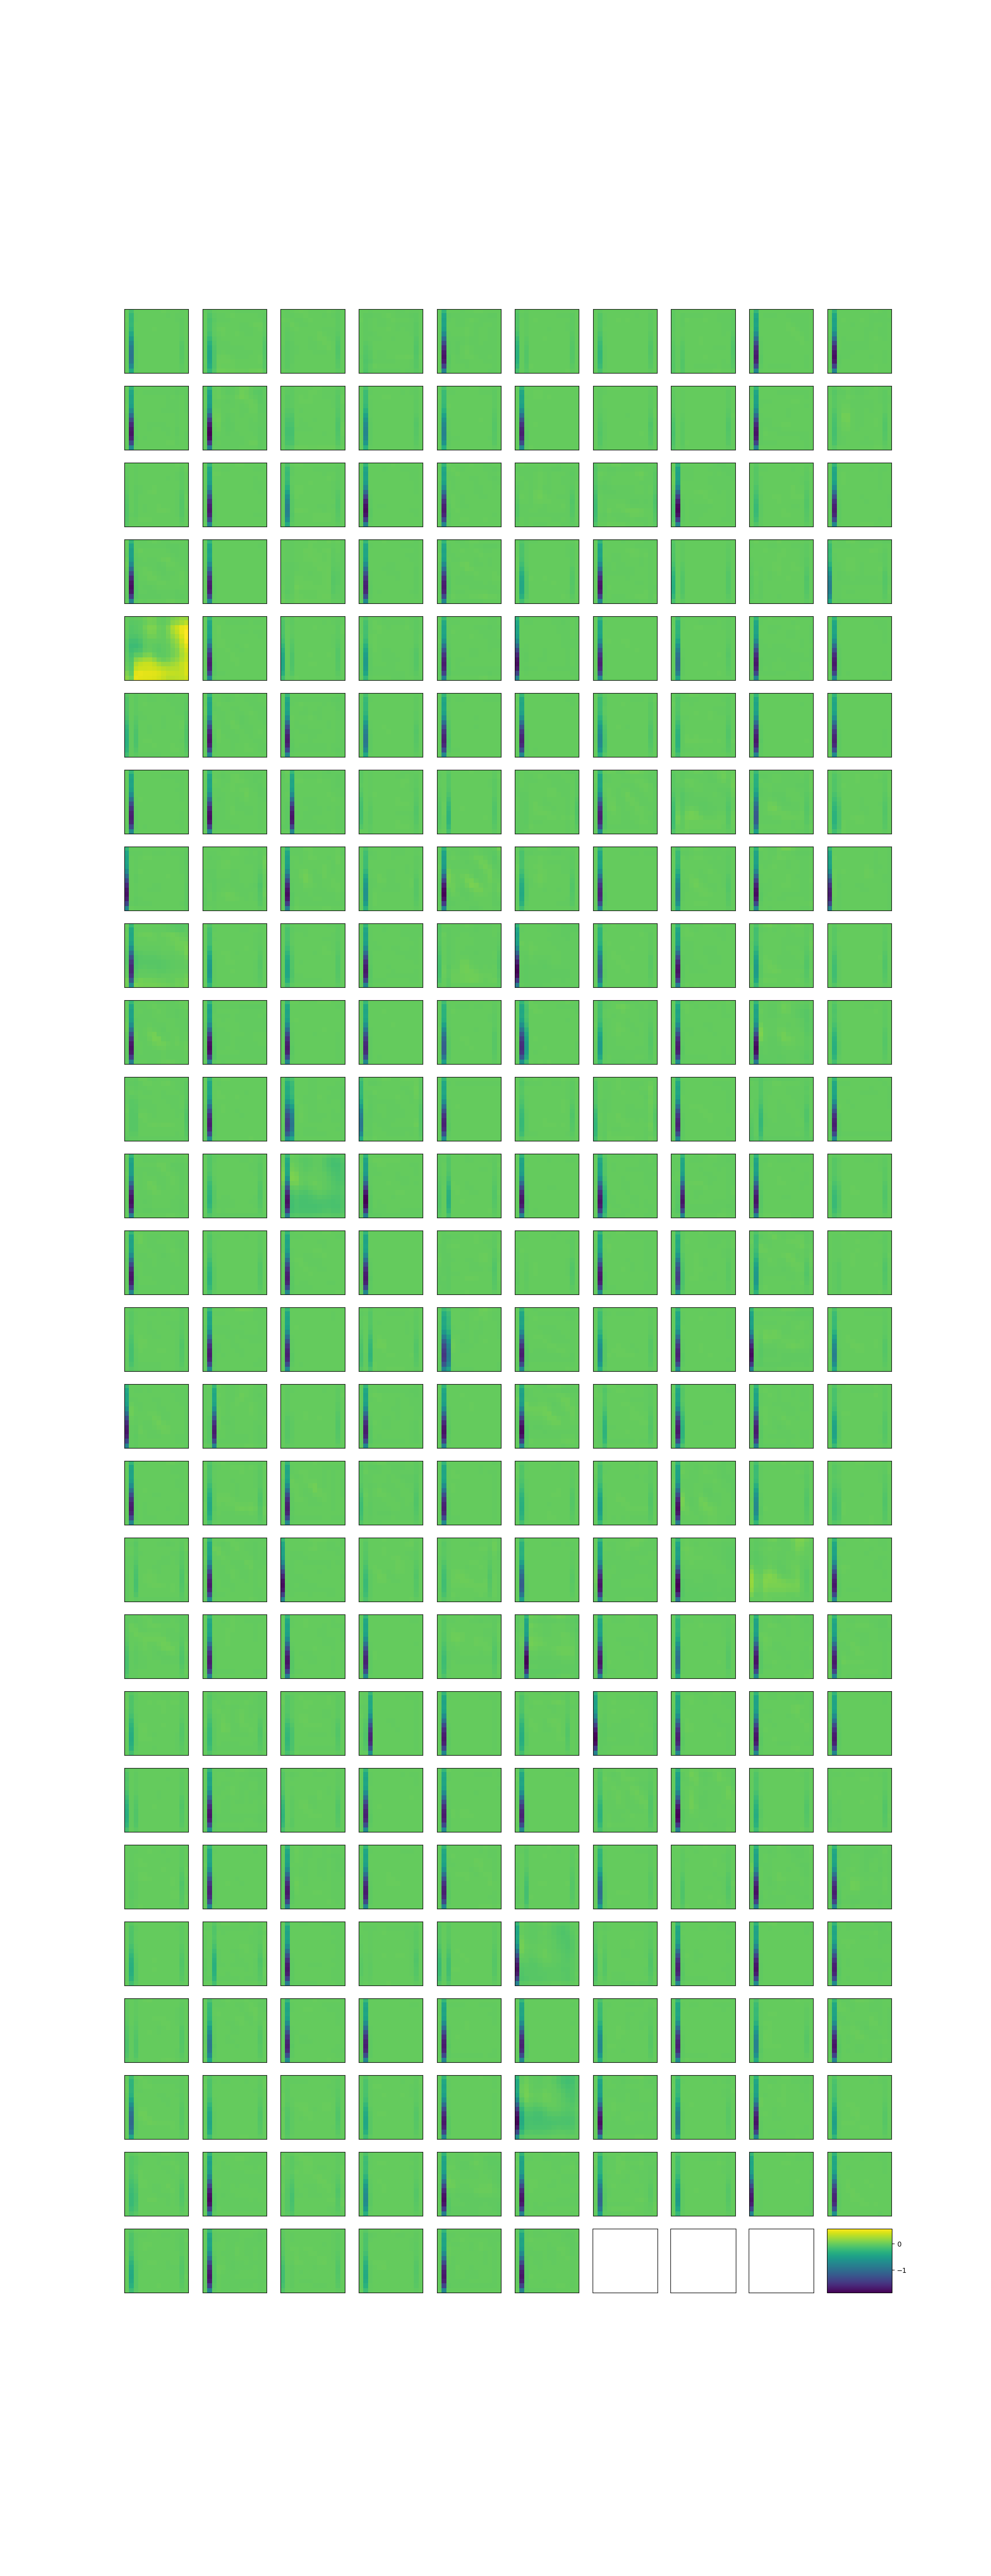
\includegraphics[width=\textwidth]{images/stripes/leaky_re_lu_5.png}
        \caption{The feature maps after LeakyReLU 5}
        \label{subfig:lakyrelu5}
    \end{subfigure}
    \hfill
    \begin{subfigure}{0.3\textwidth}
        \centering
        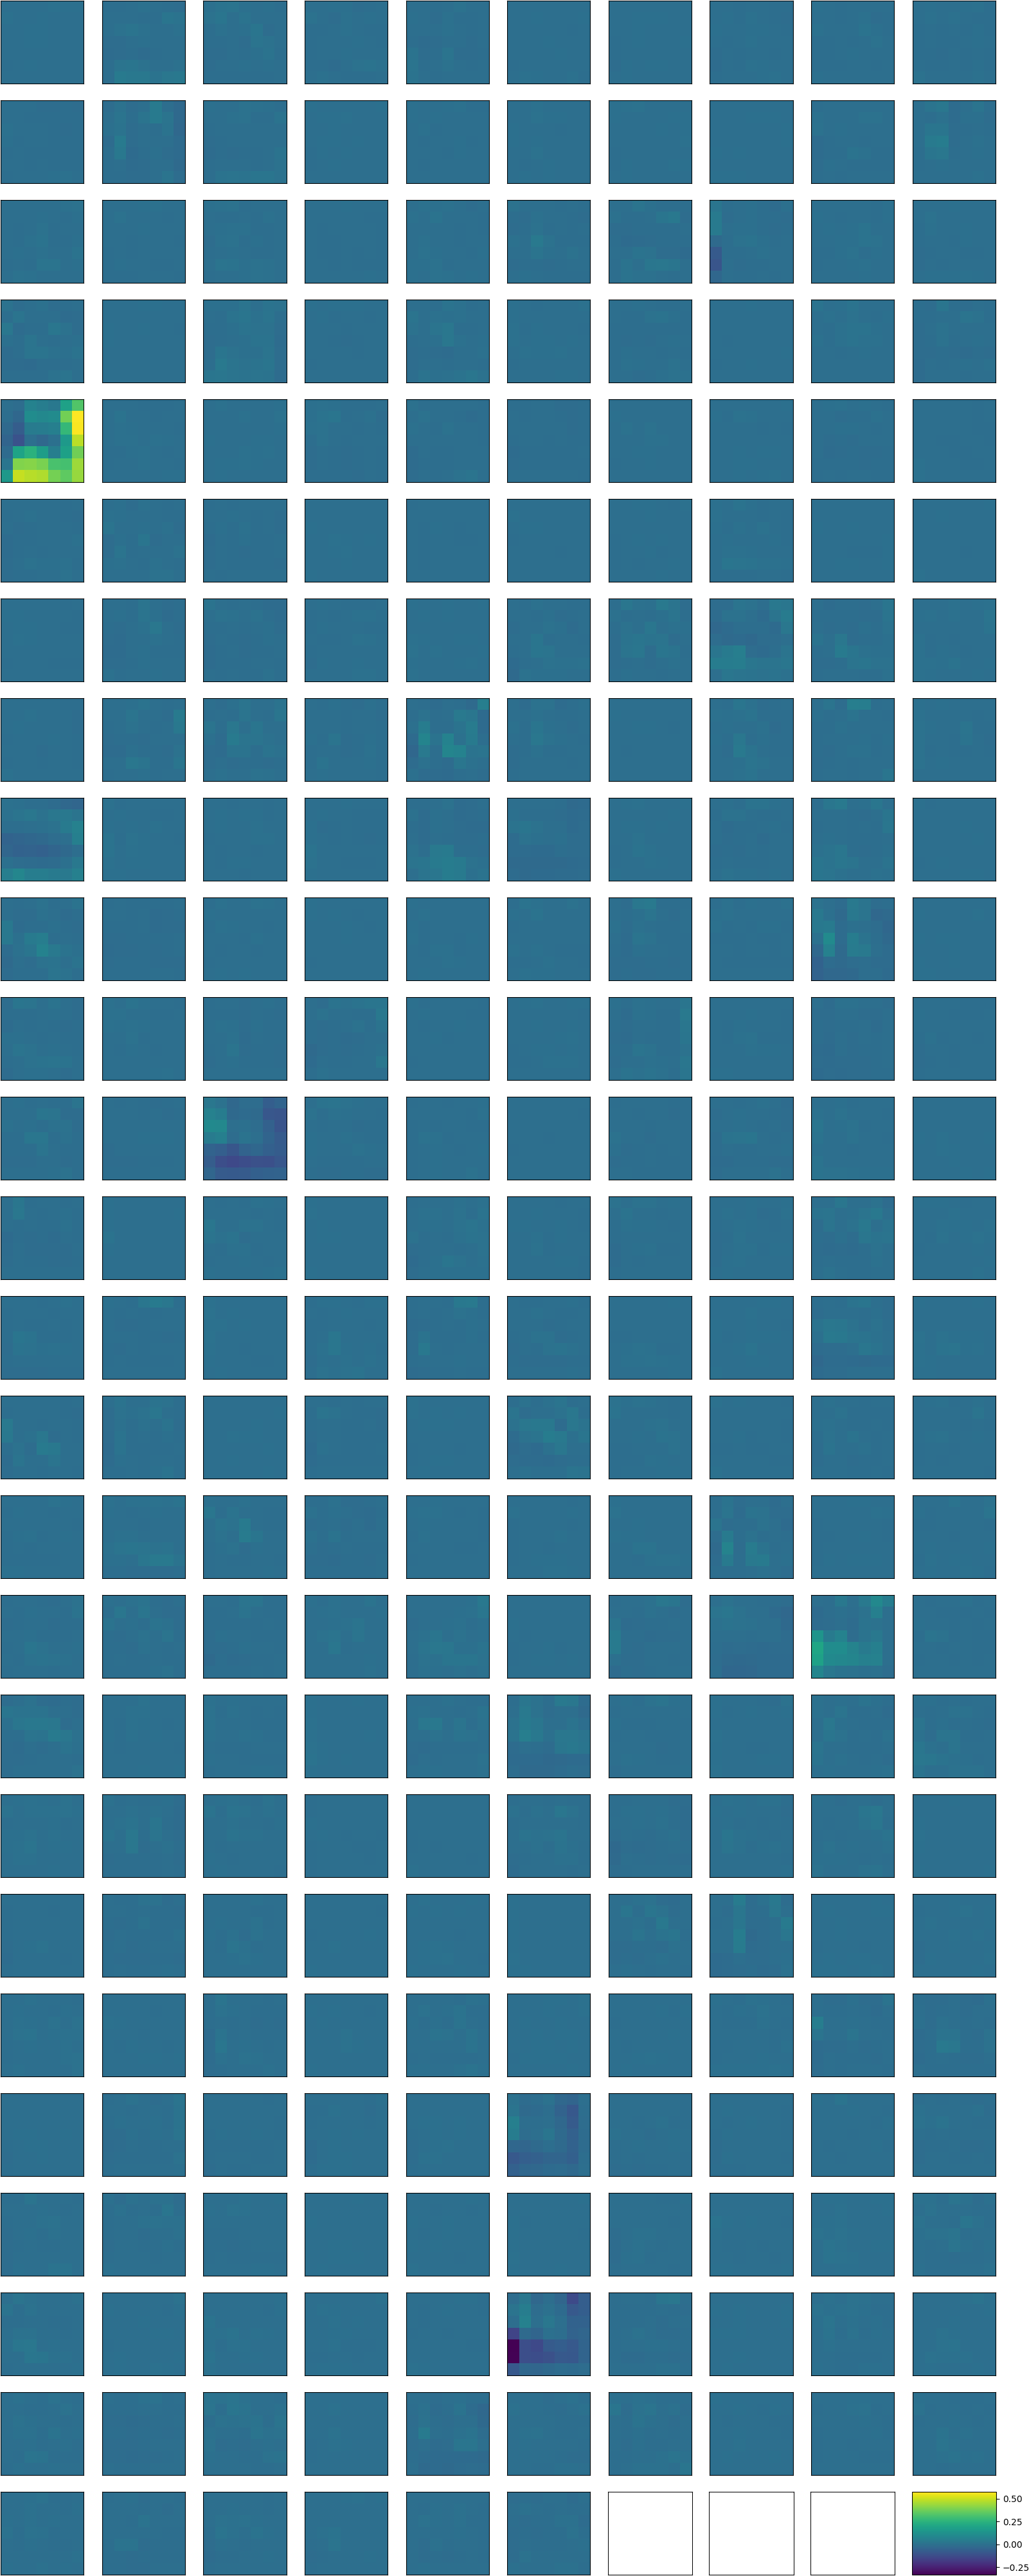
\includegraphics[width=\textwidth]{images/stripes/max_pooling2d_3.png}
        \caption{The feature maps after max pooling of LeakyReLU 5}
        \label{subfig:maxpool}
    \end{subfigure}
    \caption{The original image and the feature maps after passing the image through the network until after the specified layer. The stripe artifacts can be observed in many feature maps in Subfigure~\ref{subfig:lakyrelu5}. They vanish after max-pooling (Subfigure~\ref{subfig:maxpool}).}
    \label{fig:stripes}
\end{figure}


One observation being made during the analysis of the networks was the emergence of striped artifacts in the networks feature maps (Figure~\ref{fig:stripes}).
These stripes were observed in the Vanilla VAE, AlexNetVAE, as well as the AlexNet Classifier and might be also present in other networks (\textbf{CHECK THIS}).
Apparently, the stripes are either always horizontal or vertical for one network type.
If they are vertical, they can appear on the left or the right side of the same network.
If they are horizontal, they appear either on the top or on the bottom of the same network.
The exact reason why the networks show this behavior was not found, however some insights were won.

\paragraph{Padding}
The stripes occur due to the zero-padding in the network and the resulting contrast observed by the convolutional filters.
Take Figure~\ref{fig:stripes}.
Here, the stripes appear strongest on the bottom left of the image.
Noteworthy, the stripes indicate less active regions in the feature map: The feature map has an activity of around zero everywhere except for the location of the stripes.
Here, the activity is strongly negative.

A comparison with the original image (Figure~\ref{subfig:stripes_original}) shows that for the left side of the image, the contrast is highest on the bottom if the image is zero-padded\footnote{Zero-padding can be understood as adding black pixels around the image.}.
Importantly, the contrast is as high on the bottom of the image, the right side, and the right side of the top of the image.
However, for this network, the stripes seem to occur for a sharp shift of black on the left to white on the right.

\begin{figure}
    \centering
    \foreach \n in {0,...,11}{
        \begin{subfigure}{0.05\textwidth}
            \frame{\includegraphics[width=\textwidth]{images/stripes/test_images/original\n.jpg}}
            \caption{}
            \label{subfig:test_images_stripes\n}
        \end{subfigure}
        \hfill
    }
    \caption{The test images used to analyze the networks behavior.}
    \label{fig:test_images_stripes}
\end{figure}

To better understand the behavior, the network was applied to a set of artifical test images (Figure~\ref{fig:test_images_stripes}).
All different feature maps with respect to each image can be found in the appendix.

\begin{figure}
    \centering
    \begin{subfigure}{0.45\textwidth}
        \centering
        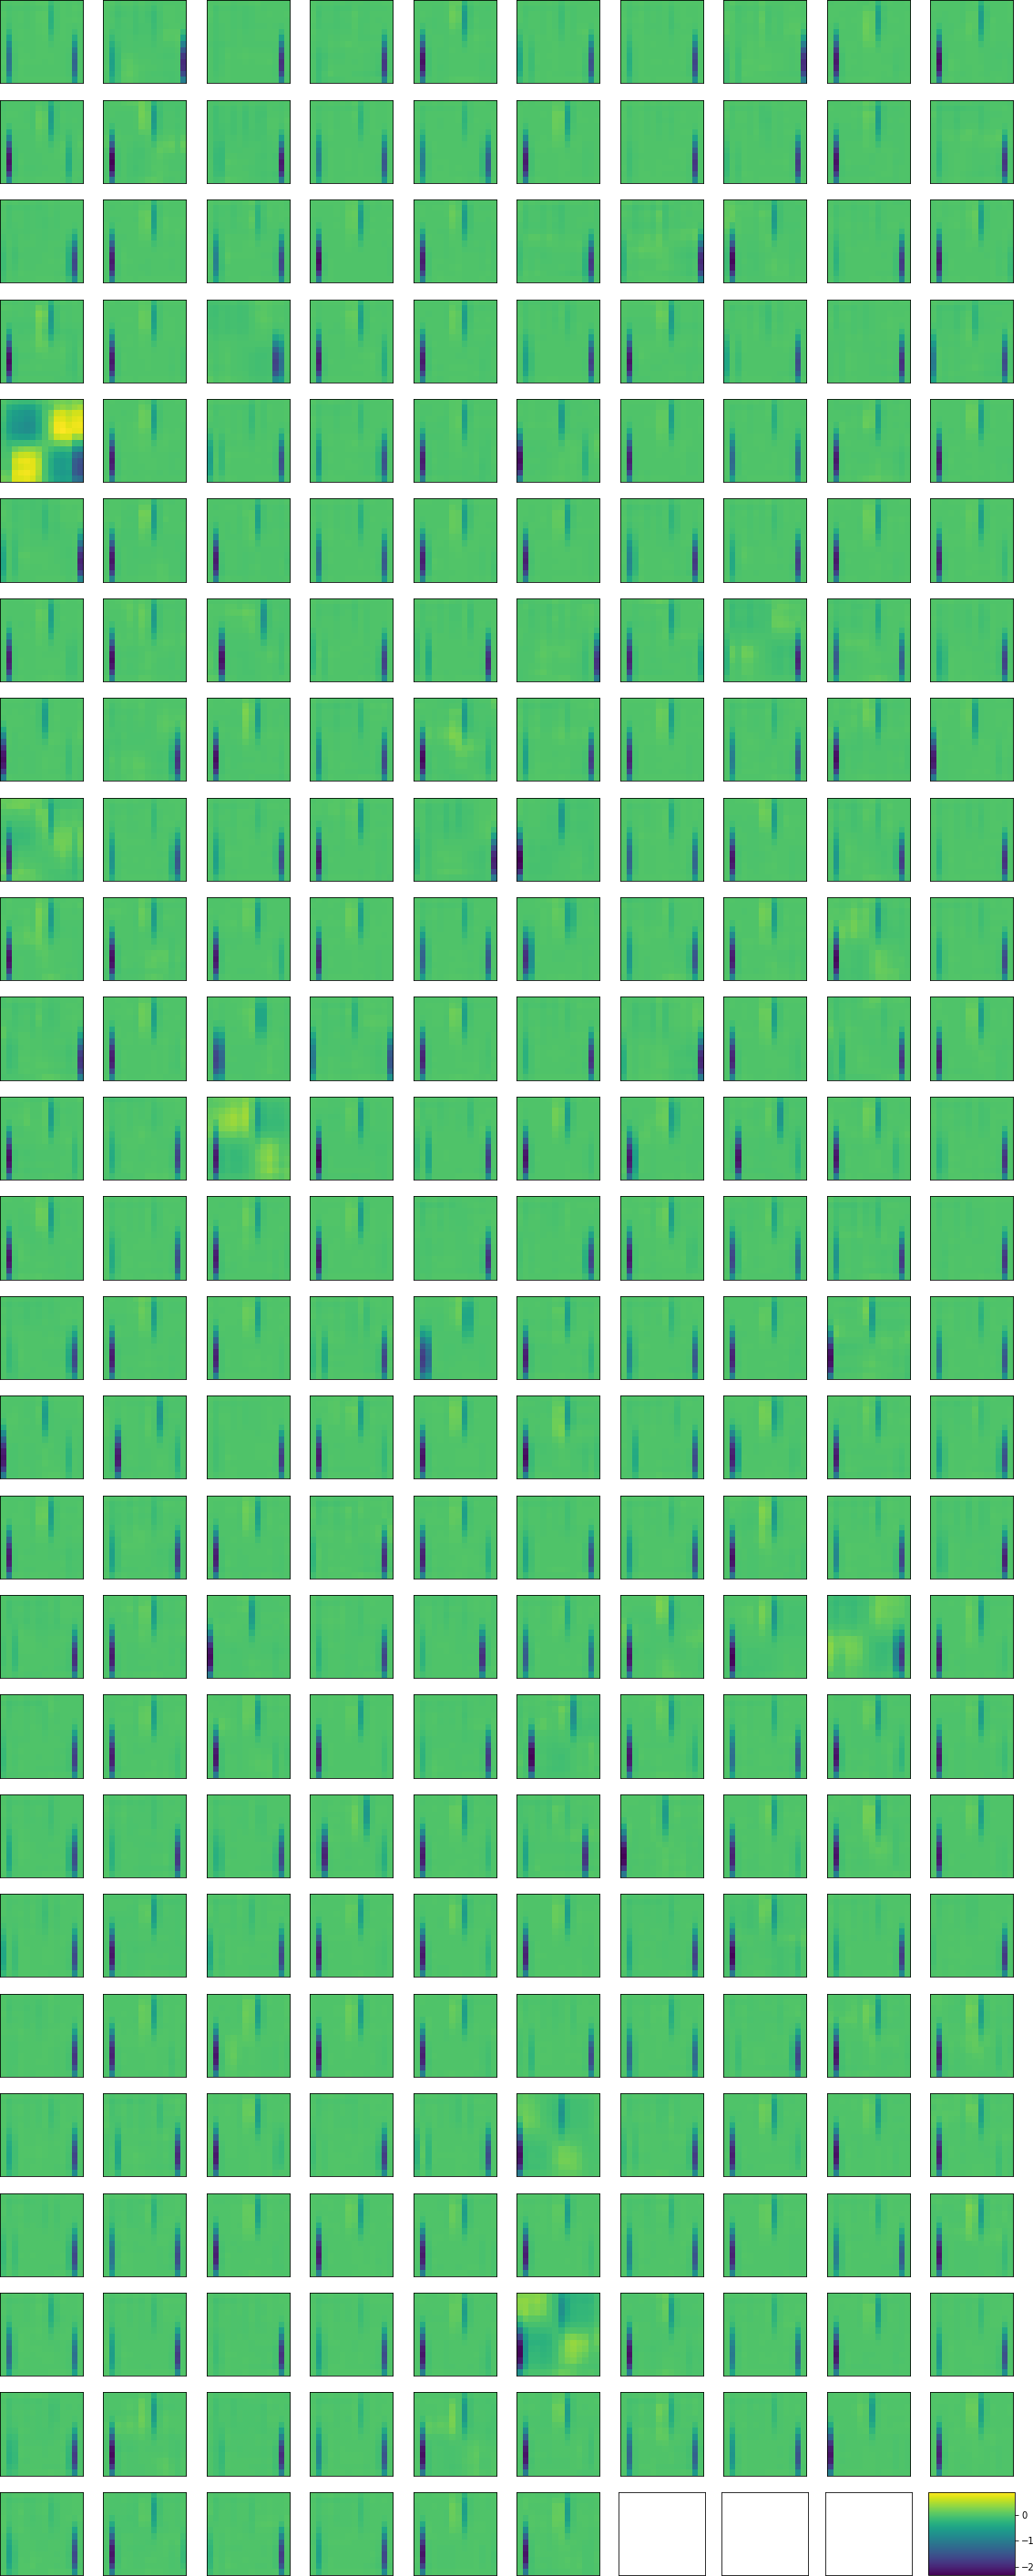
\includegraphics[width=\textwidth]{images/stripes/test_img_9/leaky_re_lu_5.png}
        \caption{The original image.}
        \label{subfig:stipes_test_img_leakyrelu5}
    \end{subfigure}
    \hfill
    \begin{subfigure}{0.45\textwidth}
        \centering
        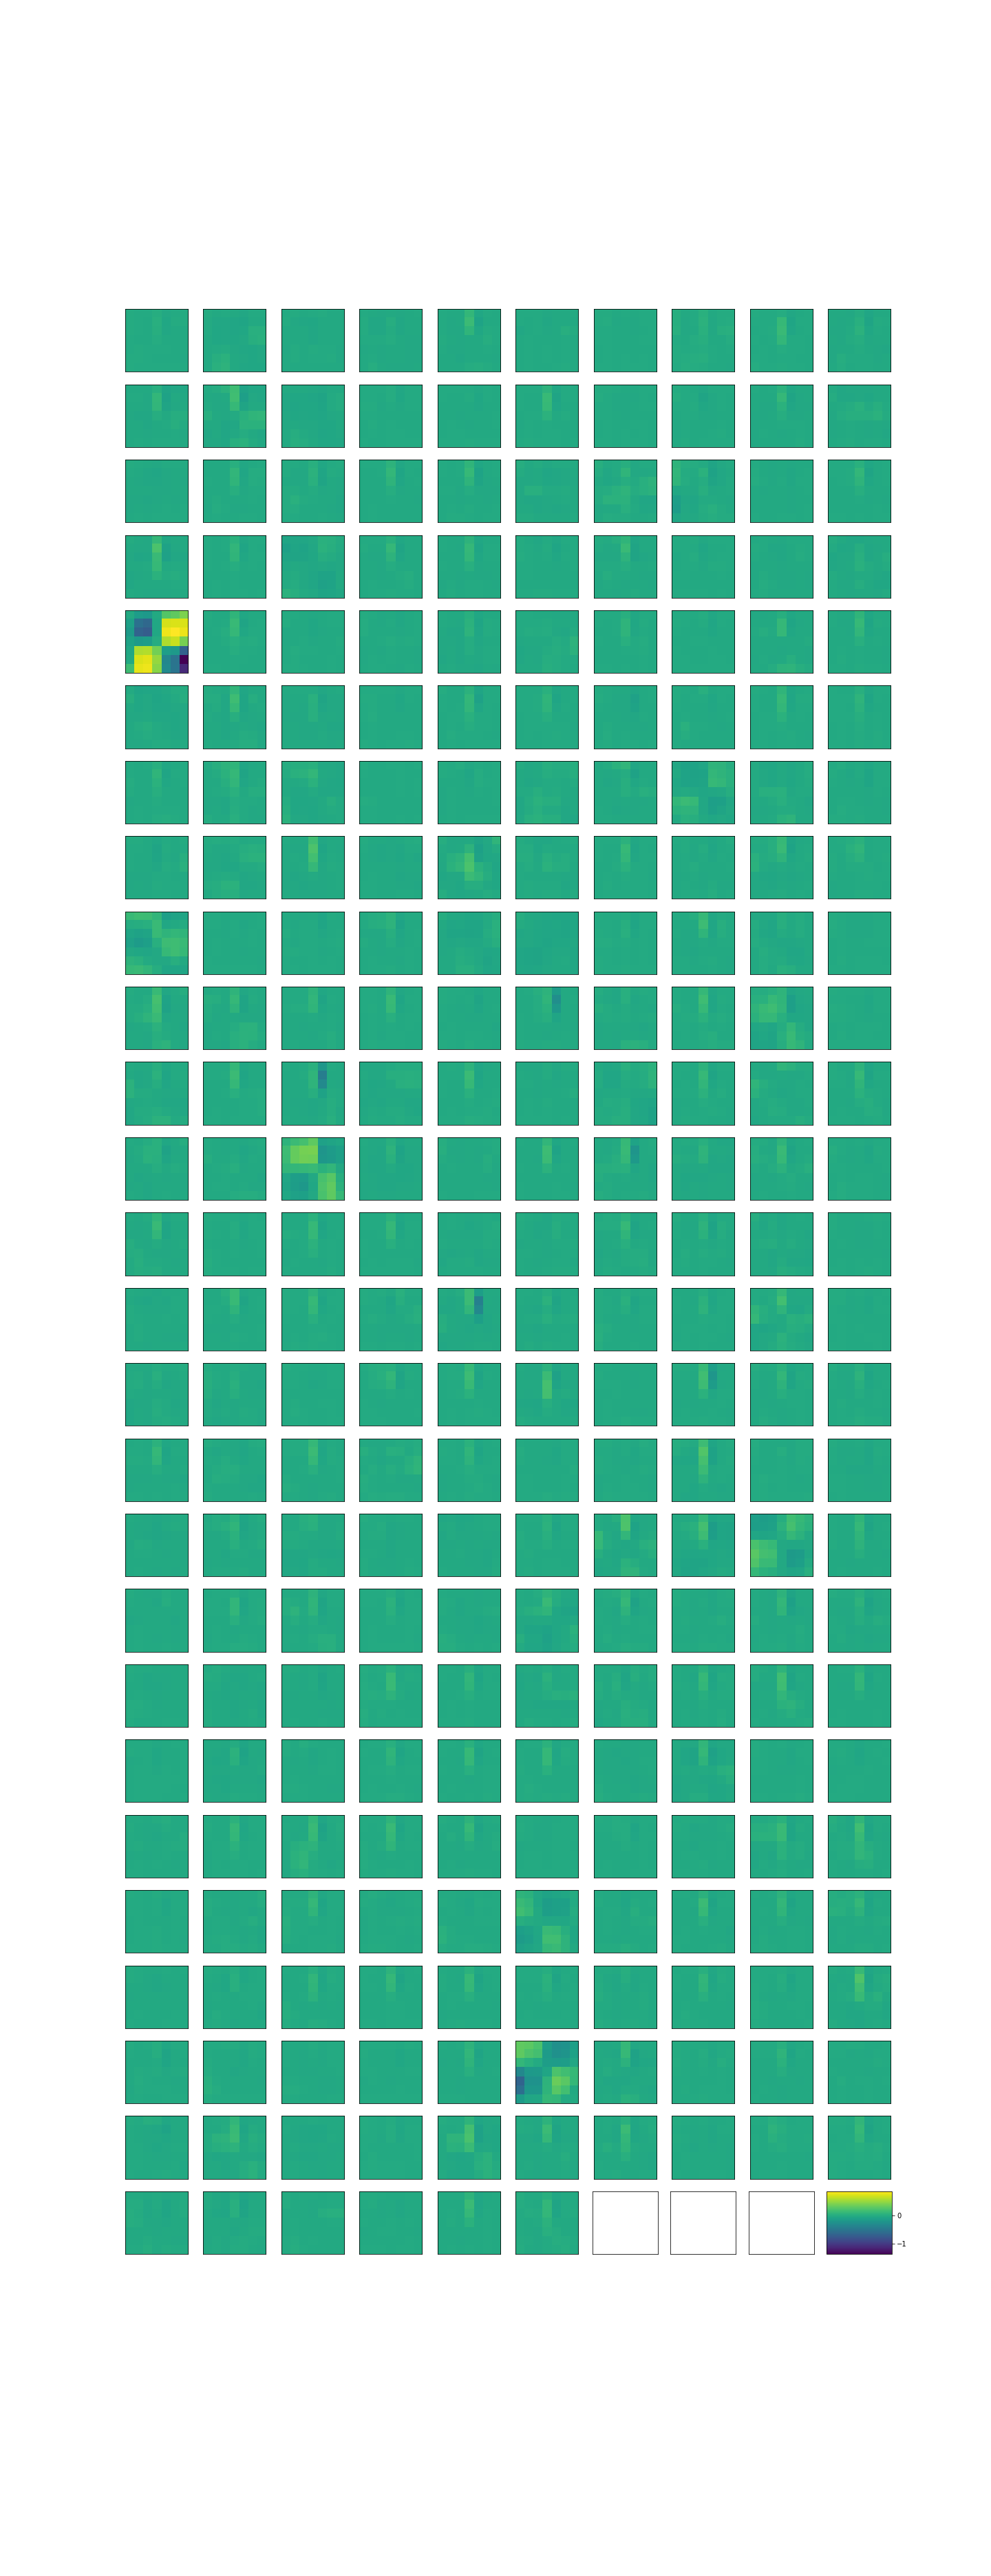
\includegraphics[width=\textwidth]{images/stripes/test_img_9/max_pooling2d_3.png}
        \caption{The feature maps after LeakyReLU 5}
        \label{subfig:stripes_test_img_maxpool3}
    \end{subfigure}
    \caption{The feature maps with respect to test image~\ref{subfig:test_images_stripes8}.}
    \label{fig:stripes_test_img}
\end{figure}

Subfigure~\ref{subfig:test_images_stripes8} and~\ref{subfig:test_images_stripes11} turned to be most equally high insightful.
Figure~\ref{fig:stripes_test_img} shows the feature map after the last LeakyReLU (LeakyReLU 5) activation of the network given this input image (Subfigure~\ref{subfig:stipes_test_img_leakyrelu5}) as well as the feature map after max-pooling of this feature map (Subfigure~\ref{subfig:stripes_test_img_maxpool3}).
Multiple things can be observed in Subfigure~\ref{subfig:stipes_test_img_leakyrelu5}.
Firstly, the feature map in the first column of the fifth row resembles the input stimulus itself.
The fact that this feature map shows most of the activity (especially after max-pooling, see Subfigure~\ref{subfig:stripes_test_img_maxpool3}) has been observed for natural images as well, however not the resemblance of the input stimulus.
Except for this feature map, stripes emerge either on the bottom of the left side or the bottom of the right side of the feature map.
For the bottom of the left side, this is where the sharp black-white contrast is.
The bottom of the right side is more complicated.
Here the test image was black and the \say{contrast} is a black-black contrast - or no contrast at all.
However, this is only true for the first feature map\footnote{The first feature maps are not shown here.}.
The following feature maps, again, are zero-padded.
However, due to the bias term in the convolutions, these might be non-zero in the bottom-right and top-left square of the image, thus leading to a contrast.
This explains why the network can be sensitive towards these black-black contrasts in the input image.

Noteworthy, if the bias term in the convolutions is removed, the black-black contrast sensitivity vanishes because the network is not able anymore to add a constant to the black pixel values on the bottom-right or top-left of the image.
For this purpose, the batch normalization has to be removed too since it uses a bias term as well.
This, however, does not qualitatively change the networks behavior on real images.

